\documentclass[12pt, a4paper]{article}
\renewcommand*\contentsname{Inhaltsverzeichnis}
\usepackage[ngerman]{babel}
\usepackage{mathptmx}
\usepackage{blindtext}
\usepackage{emptypage}
\usepackage{wrapfig}
\usepackage[pdftex]{graphicx}
\usepackage{geometry}
\usepackage{setspace}
\usepackage{hyperref}
\usepackage[version=4,arrows=pgf-filled,
textfontname=sffamily,
mathfontname=mathsf]{mhchem}
\usepackage[table]{xcolor}
\usepackage{multirow}
\usepackage[table]{xcolor}
\usepackage{array}
\usepackage{float}
\usepackage{mathcomp}
\usepackage{csquotes}
\usepackage[backend=biber,style=chem-acs,sorting=none]{biblatex}
\addbibresource{literatur.bib}  % Deine .bib-Datei einbinden

\DeclareCiteCommand{\cite}
  {\usebibmacro{prenote}}
  {\textsuperscript{\printfield{labelnumber}}}
  {\multicitedelim}
  {\usebibmacro{postnote}}


 \geometry{
 a4paper,
 total={170mm,257mm},
 left=25mm,
 top=25mm,
 }
\setstretch{1.213}


\newcommand{\datum}{\day.\month.\year}
\DeclareGraphicsExtensions{.pdf,.jpeg,.png,.jpg} 

\begin{document}


\begin{figure}
    \includegraphics[scale=0.14]{Universität_Bayreuth.svg.png}
\end{figure}


%Deckblatt

{\raggedright Universität Bayreuth\\  95447 Bayreuth}


\vspace{5cm}

\begin{center}
{\LARGE\bf{Anorganische Chemie III}} \\  
\vspace{1cm}
{\Large\bf{Metall-Organic-Framework (MOF)}}\\
\vspace{0.5cm}
{\large Justus Friedrich\\}
{Studiengang: B.Sc. Chemie\\}
{4. Fachsemester}
\end{center}





\thispagestyle{empty}
\begin{center}
{\small Matrikelnummer: 1956010 \\
E–Mail:  bt725206@myubt.de}
\end{center}

\vspace{5cm}

\today


\newpage
%Inhaltsverzeichnis
\tableofcontents
\thispagestyle{empty}


%Teil 1
\newpage
\setcounter{page}{1}
\section{Einleitung}



\subsection{Einführung}
{MOFs gehören zu den Mikroporösen Materialien und werden nicht nur wegen ihrer hohen Gas adsorbier Fähigkeit und ihrer Möglichkeit als Katalysator 
immer Relevanter. Daher wird in der letzten Zeit sehr aktive Forschung an MOFs.\cite{ThomasHillman.2018}

}

\subsection{Ziel des Versuchs}
{Das Ziel dieses Versuchs ist es in einer 2er-Gruppe 4 verschiedene MOFs herzustellen. Diese werden dann miteinander verglichen und die Struktur mittels eines 
Pulverdiffraktogramms untersucht. Außerdem wird das Adsorbier-Verhalten in eine Iodkammer untersucht



}

\newpage
%Teil2
\renewcommand{\arraystretch}{1.3}
\section{Durchführung}
\subsection{Durchführung}
Es werden, um den entsprechenden MOF herzustellen, der Linker und das Metallchlorid werden in den Mengen die die Tabelle \ref{MOFmengen} beschreibt in 5 mL Dimethylformamid gelöst. 
Die Lösung wird dann in einen Autoklav überführt, und für 30 min bei 140 °C bei autogenen Druck zur Reaktion gebracht

\begin{table}[h!]
\caption{\textit{Zeigt die benötigten Reaktanten für die Synthese von Al-MIl-53-H, Fe-MIl-53-H, Al-MIl-53-NH$_2$, Fe-MIl-53-NH$_2$}.\cite{Skript}}
\begin{center}
\begin{tabular}{|>{\columncolor{lime}}p{4cm}|p{4cm}|p{6cm}|}
    \hline
    \rowcolor{gray}
    MOF & Einwaage $MCL_3$ & Einwaage Linker \\
    \hline
    Al-MIl-53-H & 123.4 mg $AlCl_3$ & 172.3 mg Terephtalsäure \\
    \hline
    Fe-MIl-53-H & 138.2 mg $FeCl_3$ & 172.3 mg Terephtalsäure\\
    \hline
    Al-MIl-53-NH$_2$ & 123.4 mg $AlCl_3$ & 187.8 mg Aminoterephtalsäure\\
    \hline
    Fe-MIl-53-NH$_2$ & 138.2 mg $FeCl_3$ & 187.8 mg Aminoterephtalsäure\\
    \hline

\end{tabular}

\end{center}
\label{MOFmengen}

\end{table}
\noindent
{
Das entstandene Produkt wird in ein Zentrifugenglas überführt, und für 5 min bei 5000 
Umdrehungen die Minute zentrifugiert. Das DMF wird dekantiert und entsorgt. 
Anschließend wird das Produkt mit Wasser 
aufgeschwemmt und erneut zentrifugiert und dekantiert. 
Der Prozess wird mit Ethanol wiederholt. Nachdem das Ethanol abdekantiert ist, wird das Produkt im Trockenschrank getrocknet.\cite{Skript}
\vspace{0.2cm}}\\
{
Vom dem MOFs werden XRDs augenommen. Anschließend wird eine Spatelspitze der MOFs in ein Rollglas gegeben und mit etwas Iod auf 50 °C 
erhitzt. Dabei wird das Verhalten beobachtet.
}

\newpage
\section{Auswertung}
\subsection{Porenanalyse MOFs}
\subsubsection{Porenanalyse Porenanalyse}
Um zu bestimmen, ob das MOF Al-MIL-53-H im Large-Pore- oder im Narrow-Pore-Typ vorliegt, wird das aufgenommene Pulverdiffraktogramm mit Referenzmustern verglichen. 
Dieser Vergleich ist in Abbildung \ref{MOF125ver} dargestellt.
\begin{figure}[!ht]
    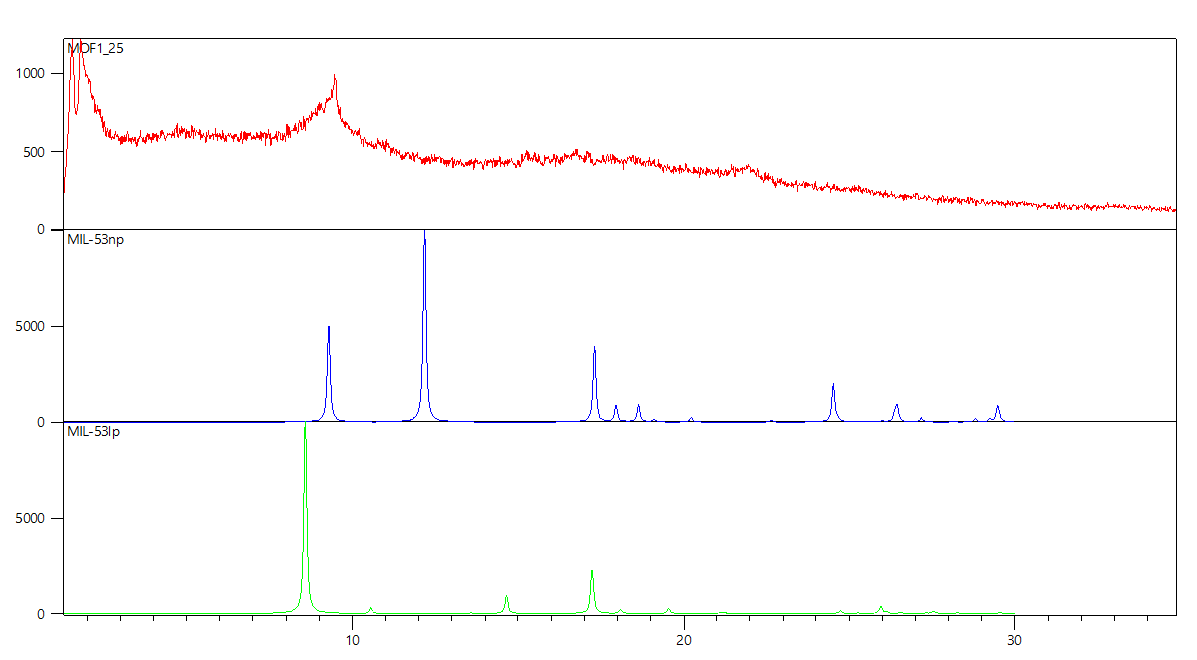
\includegraphics[scale=0.5]{MOF125ver.png}
    \caption{\textit{Es wird das Pulverdiffraktogramm von Al-MIL-53-H (rot) und die Referenzreflexe von MIL-53 narrow-pore (blau) Large-pore(grün) abgebildet}}
    \label{MOF125ver}
\end{figure}

\noindent
Aus Abbildung \ref{MOF125ver} lässt sich der Porentyp des hergestellten MOFs aufgrund der schwachen Reflexe nur schwer eindeutig bestimmen. 
Allerdings scheint eine bessere Übereinstimmung der Reflexe mit denen des Narrow-Pore-Typs vorzuliegen. 
Daher wird das hergestellte MOF Al-MIL-53-H dem Narrow-Pore-Typ zugeordnet.

\subsubsection{Porenanalyse Fe-MIl-53-H}
In Abbildung \ref{MOF120ver} ist das Pulverdiffraktogramm von Fe-MIL-53-H zusammen mit den Referenzmustern dargestellt. Auch in diesem Fall ist eine eindeutige Zuordnung der Reflexe schwierig. 
Mithilfe der im Programm HighScore Plus generierten Peakliste (Reflexe bei 9.02°, 16.47° und 18.13°) lassen sich die Peaks jedoch dem Large-Pore-Typ zuordnen.
\newpage
\begin{figure}[!ht]
    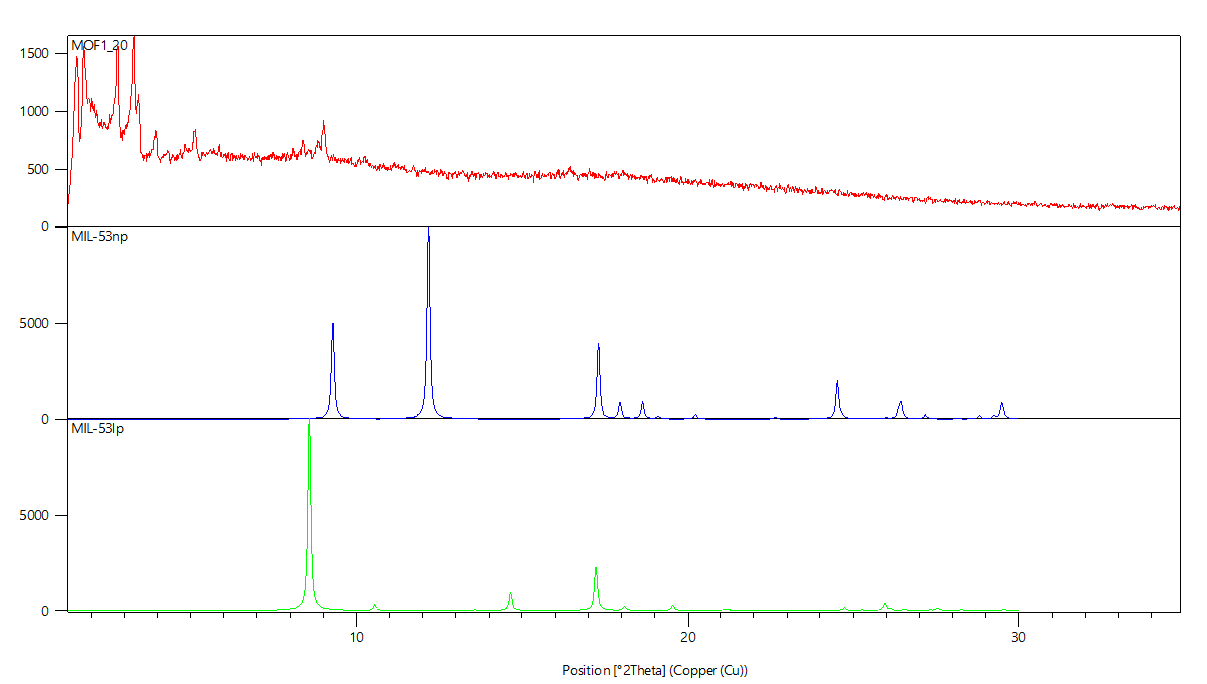
\includegraphics[scale=0.5]{MOF120ver.png}
    \caption{\textit{Es wird das Pulverdiffraktogramm von Fe-MIl-53-H (rot) und die Referenzreflexe von MIL-53 narrow-pore (blau) und Large-pore (grün) abgebildet}}
    \label{MOF120ver}
\end{figure}

\subsubsection{\texorpdfstring{Porenanalyse Al-MIl-53-NH$_2$}{Porenanalyse Al-MIl-53-NH2}}

In Abbildung \ref{MOF225ver} ist das Pulverdiffraktogramm von Al-MIL-53-NH$_2$ gemeinsam mit den Referenzmustern dargestellt. 
\begin{figure}[!h]
    \centering
    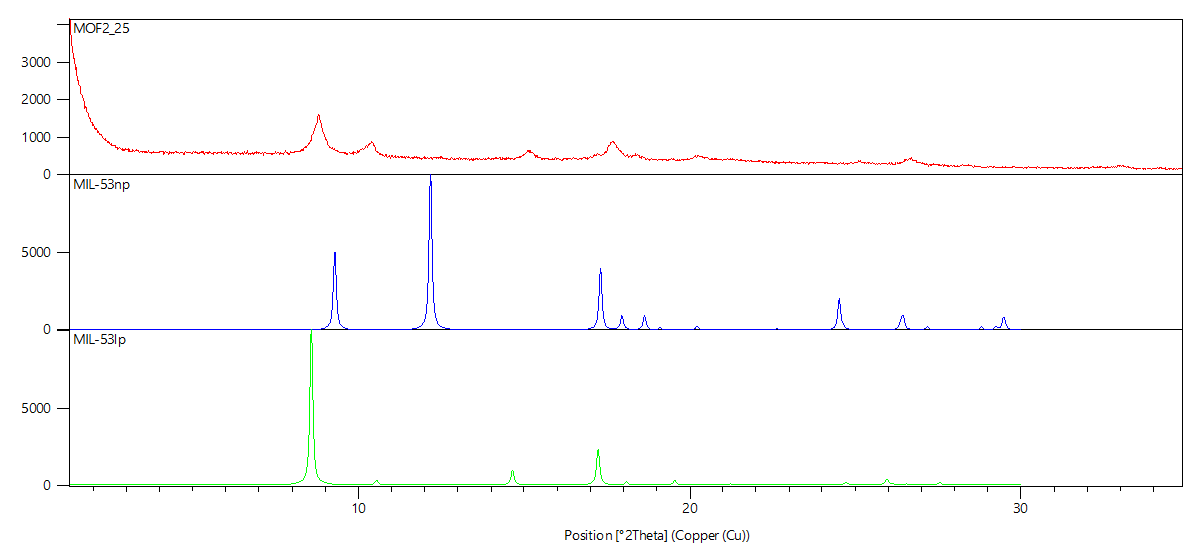
\includegraphics[scale=0.5]{MOF225ver.png}
    \caption{\textit{Es wird das Pulverdiffraktogramm von Al-MIl-53-NH$_2$ (rot) und die Referenzreflexe von MIL-53 narrow-pore (blau) und Large-pore (grün) abgebildet}}
    \label{MOF225ver}
\end{figure}
Aus Abbildung \ref{MOF225ver} geht hervor, dass Al-MIL-53-NH$_2$ in der Large-Pore-Konformation vorliegt. Dies lässt sich anhand der Übereinstimmung der gemessenen Reflexe mit denen des Large-Pore-Referenzmusters erkennen.

\newpage

\subsubsection{\texorpdfstring{Porenanalyse Fe-MIl-53-NH$_2$}{Porenanalyse Fe-MIl-53-NH2}}
In Abbildung \ref{MOF220ver} ist das Pulverdiffraktogramm von Fe-MIL-53-NH$_2$ gemeinsam mit den Referenzmustern dargestellt. 

\begin{figure}[!h]
    \centering
    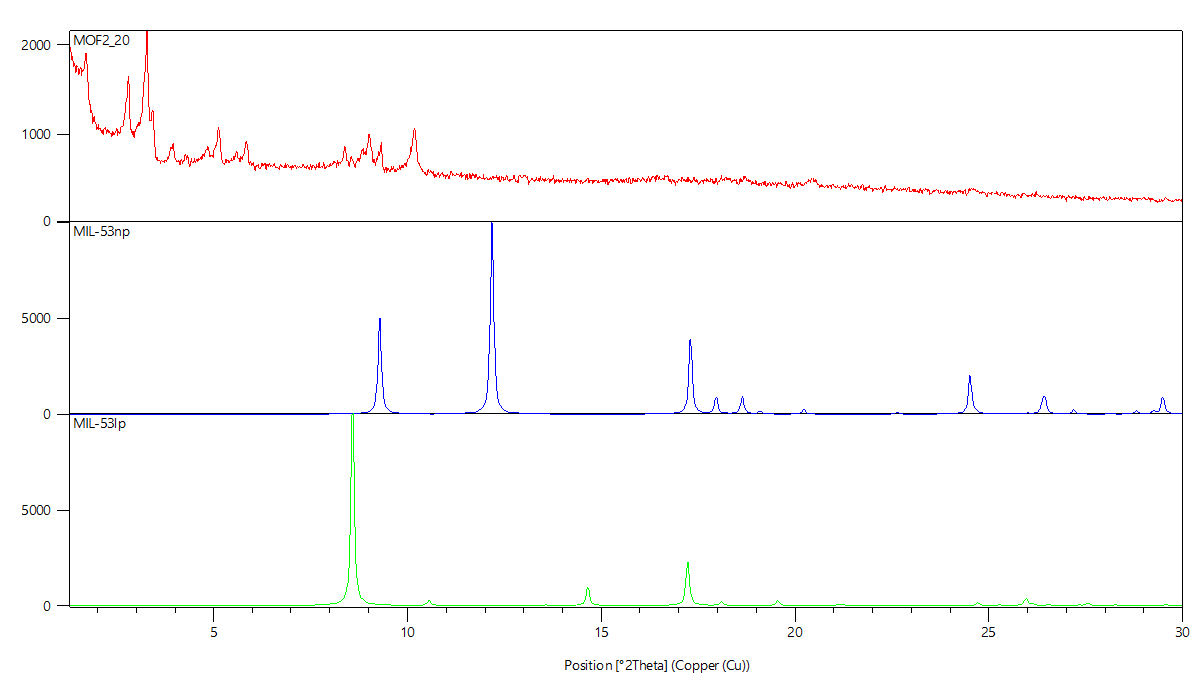
\includegraphics[scale=0.5]{MOF220ver.png}
    \caption{\textit{Es wird das Pulverdiffraktogramm von Al-MIl-53-NH$_2$ (rot) und die Referenzreflexe von MIL-53 narrow-pore (blau) und Large-pore (grün) abgebildet}}
    \label{MOF220ver}
\end{figure}
\noindent
Aus Abbildung \ref{MOF220ver} lässt sich nicht eindeutig erkennen, ob das MOF in der Narrow-Pore- oder in der Large-Pore-Konformation vorliegt. Die im Programm erstellte 
Peakliste liefert jedoch Hinweise auf die Large-Pore-Anordnung, da kleinere Reflexe bei 9.33°, 10.18°, 16.53° und 18.72° auftreten.


\newpage
\section{Zusammenfassung}



\newpage
\section{Literaturverzeichnis}
\printbibliography


\end{document}